\documentclass[12pt,a4paper]{article}
\usepackage[utf8]{inputenc}
\usepackage[margin=2.5cm]{geometry}
\usepackage{amsmath}
\usepackage{amsfonts}
\usepackage{amssymb}
\usepackage{graphicx}
\usepackage{float}
\usepackage{booktabs}
\usepackage{array}
\usepackage{multirow}
\usepackage{url}
\usepackage{hyperref}
\usepackage{siunitx}
\usepackage{caption}
\usepackage{subcaption}

% Configure hyperref
\hypersetup{
    colorlinks=true,
    linkcolor=black,
    filecolor=magenta,      
    urlcolor=blue,
    citecolor=black,
}

% Configure siunitx for proper unit formatting
\sisetup{
    separate-uncertainty = true,
    multi-part-units = repeat
}

\title{\textbf{Final Tables and Analysis for Physics IA\\Chamber Pressure and Specific Impulse}}
\author{Updated Analysis with Error Bounds}
\date{\today}

\begin{document}

\maketitle

\section{Complete Measurements Table}

The complete measurements table shows all experimental trials for each pump setting, with Peak Start, Peak End, and Peak Height measurements.

\begin{figure}[H]
\centering
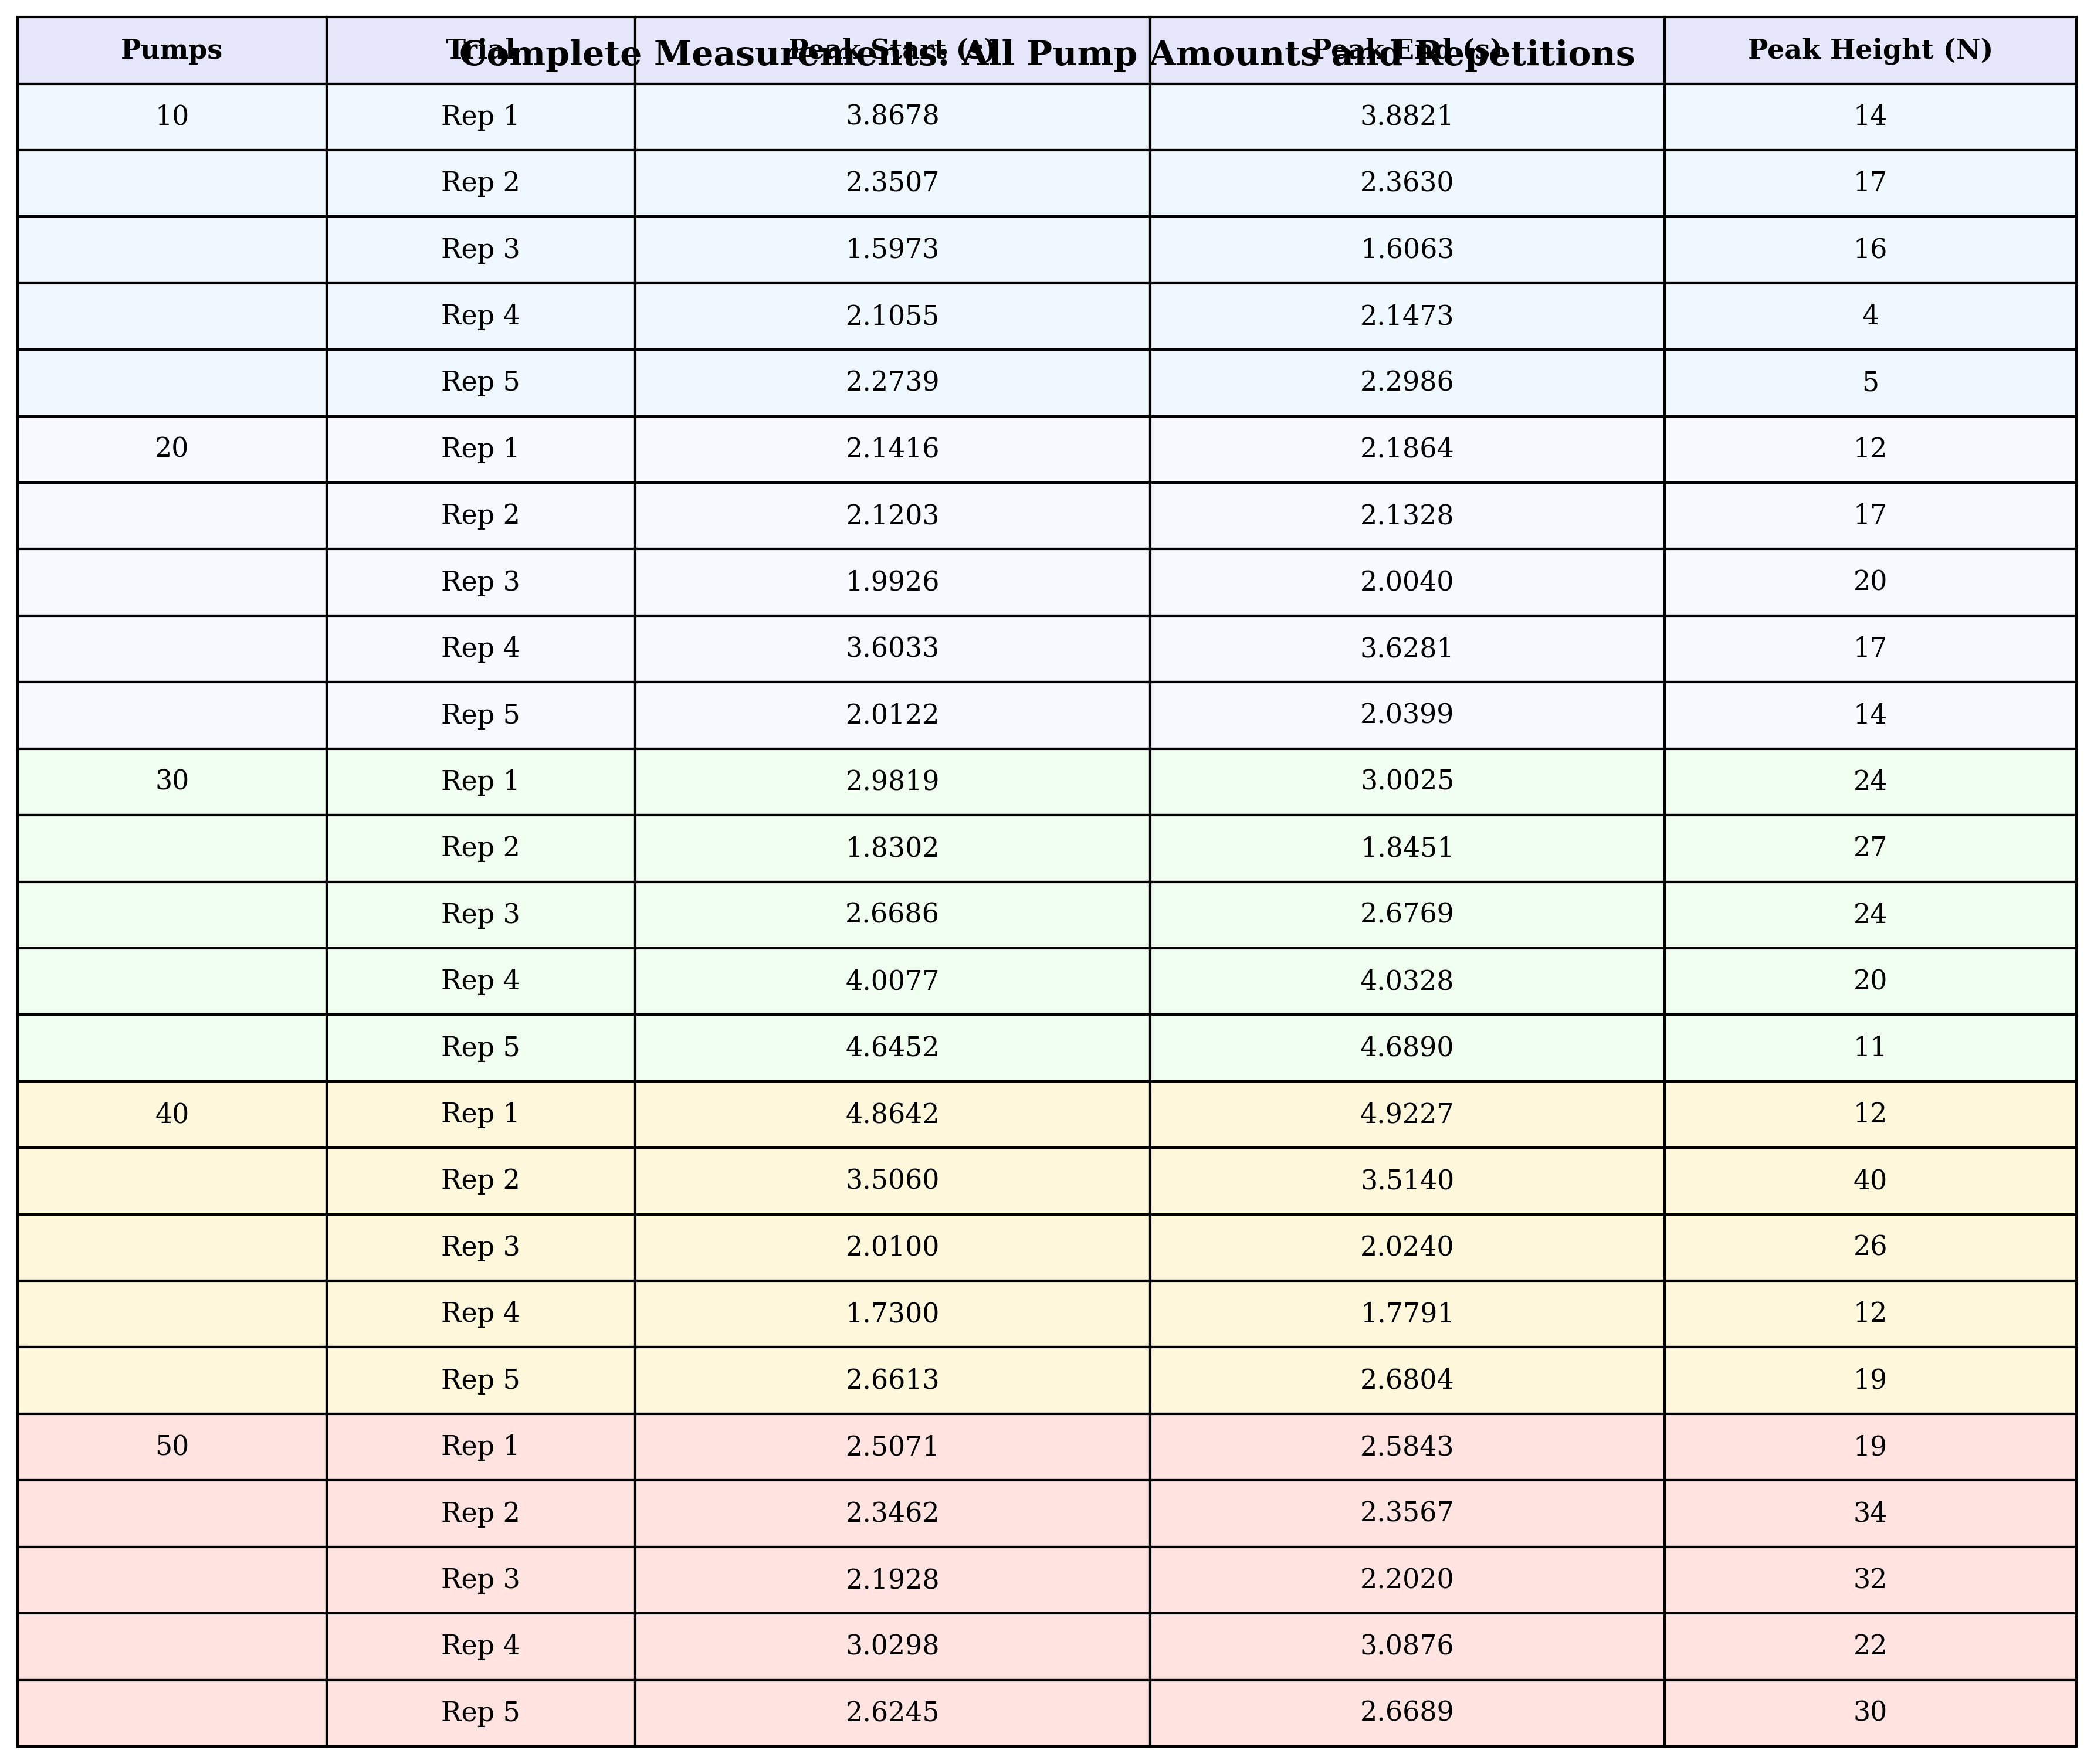
\includegraphics[width=0.95\textwidth]{complete_measurements_table.png}
\caption{Complete measurements table showing all repetitions for each pump setting (10-50 pumps)}
\label{fig:complete_measurements}
\end{figure}

\section{Pressure Analysis}

The pressure measurements table includes calculated pressures with absolute uncertainties for each pump setting.

\begin{figure}[H]
\centering
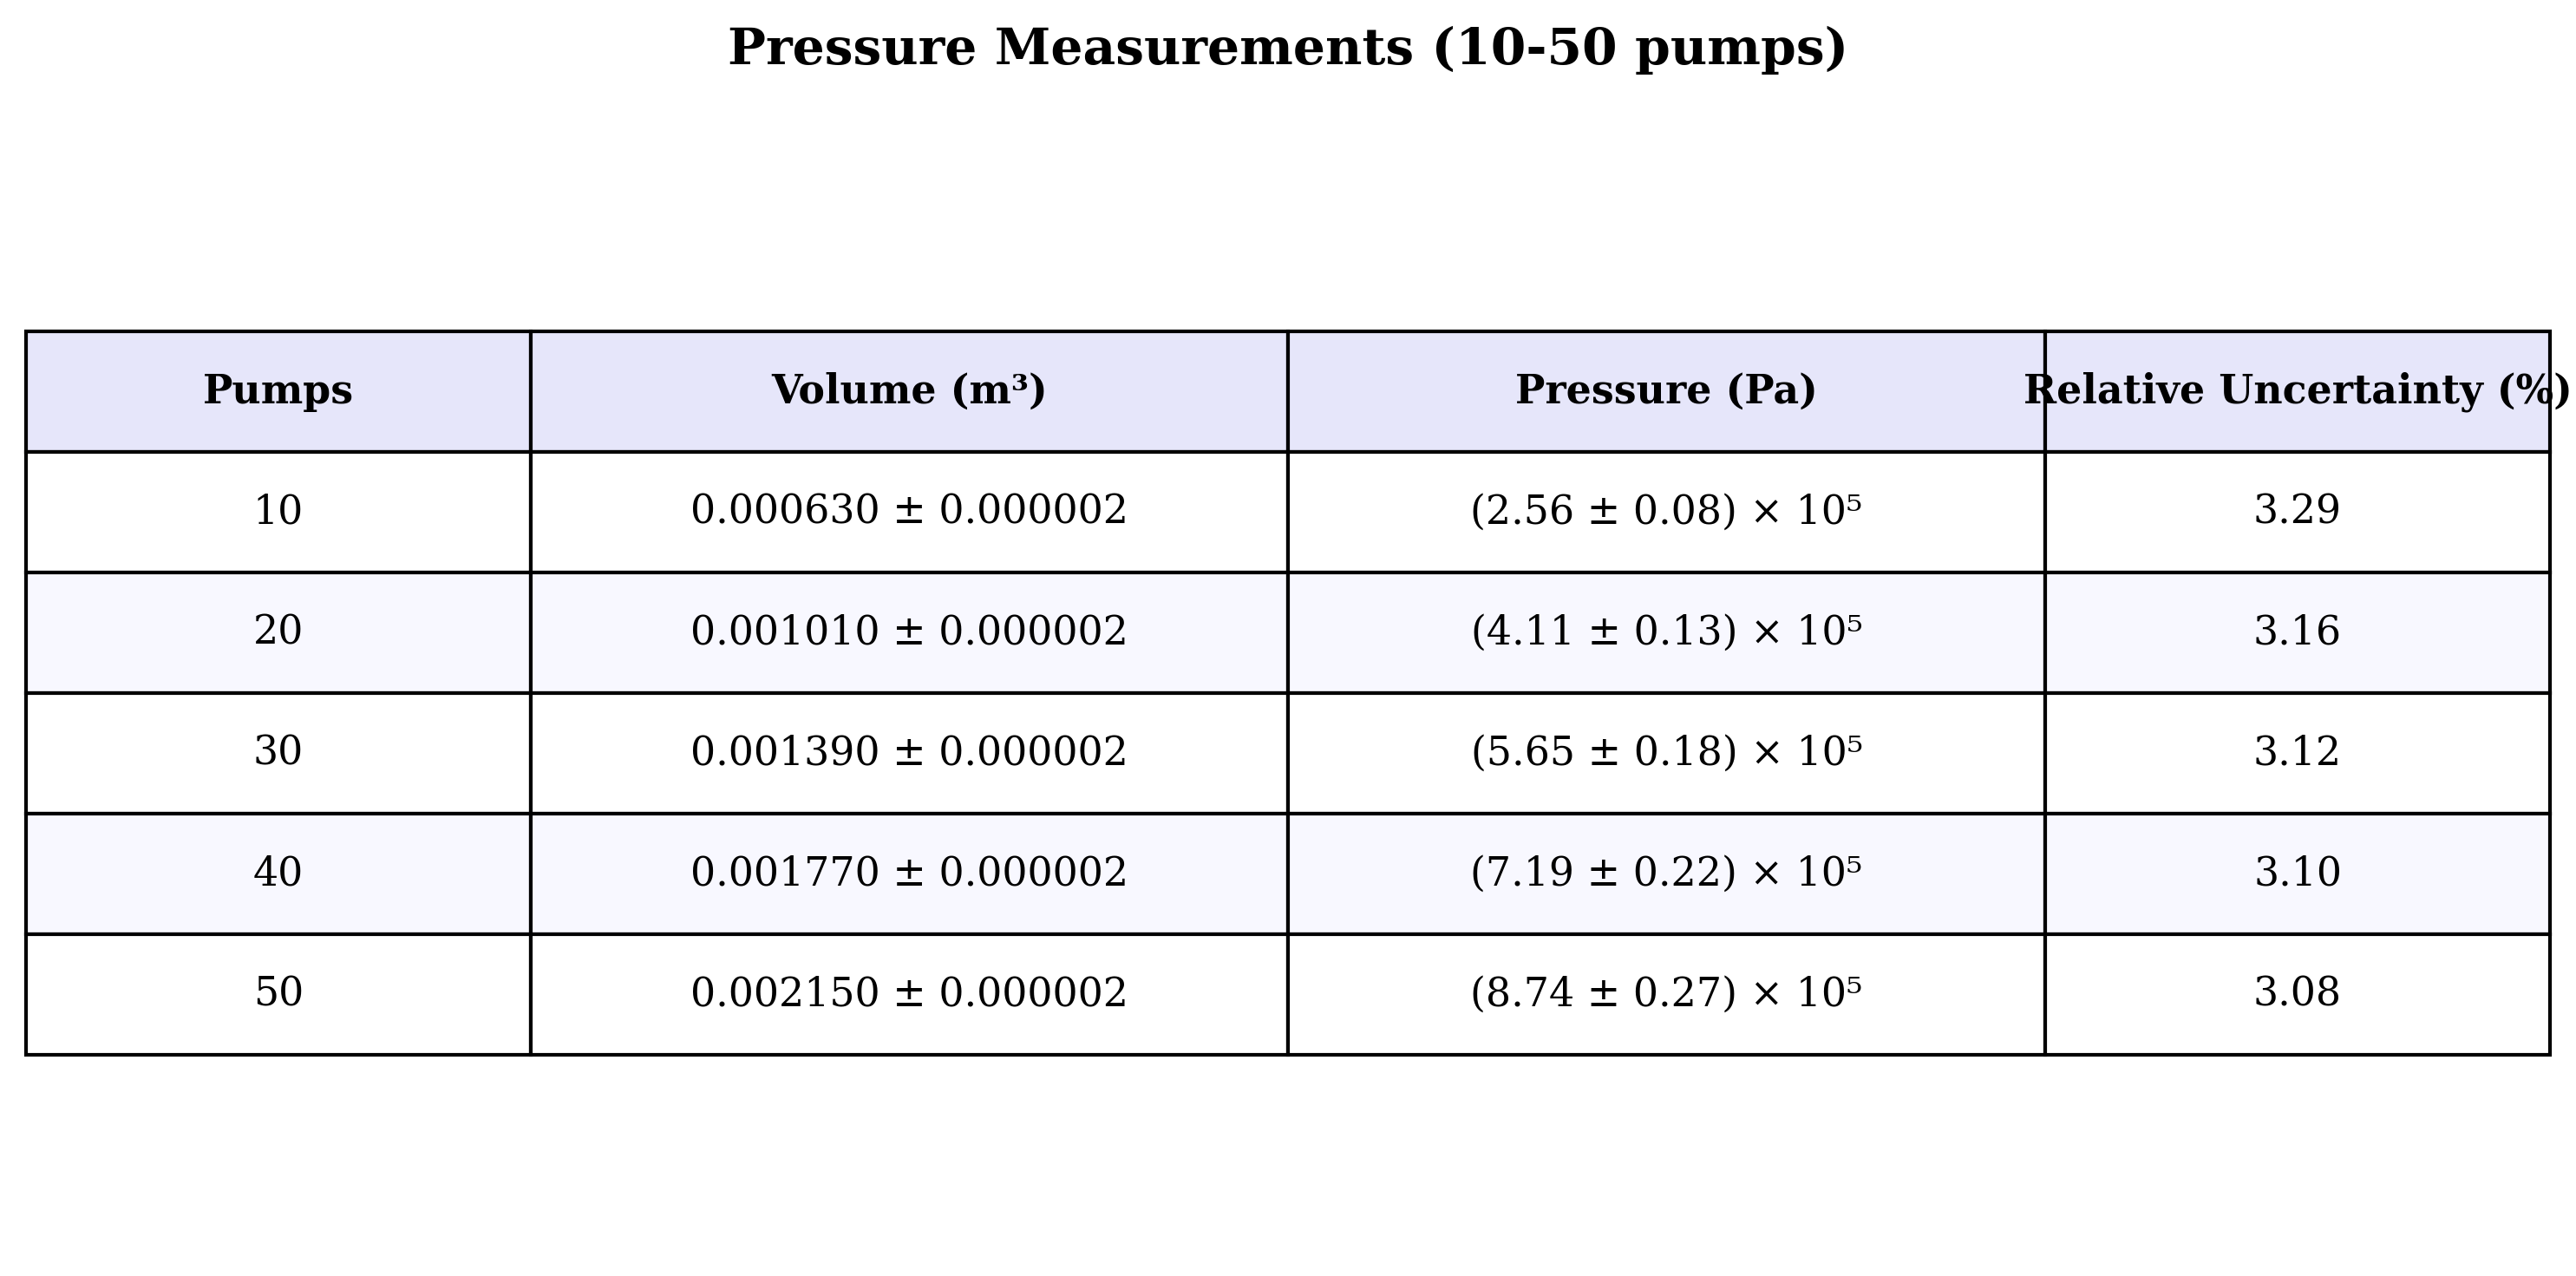
\includegraphics[width=0.9\textwidth]{pressure_table_updated.png}
\caption{Pressure measurements with absolute uncertainties for pump settings from 10-50}
\label{fig:pressure_table}
\end{figure}

\section{Impulse Analysis}

The impulse summary table shows the calculated impulse values, uncertainties, and ranges for each pump setting.

\begin{figure}[H]
\centering
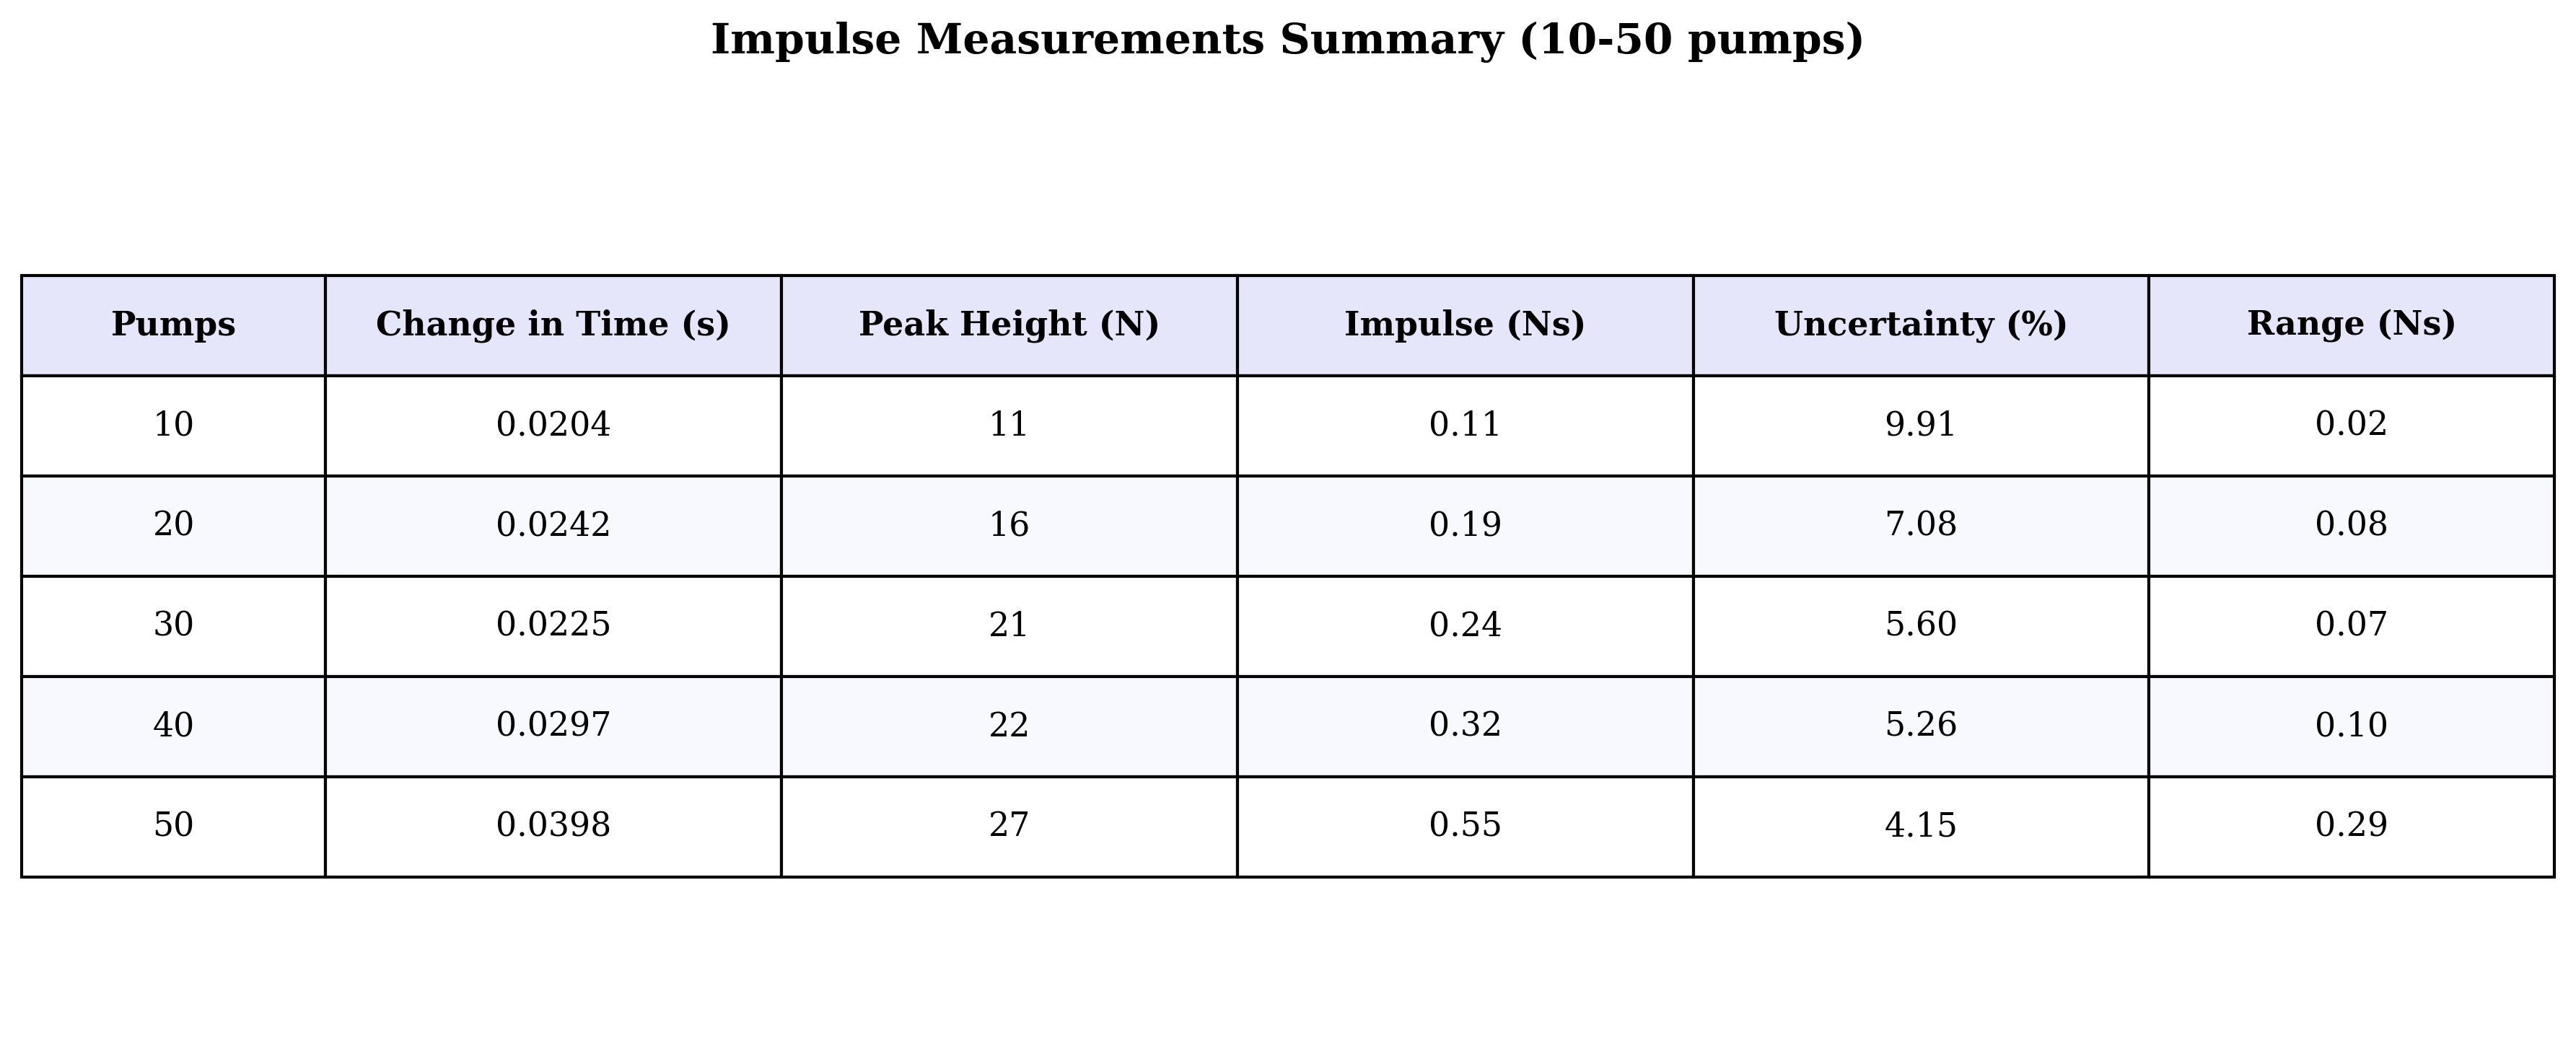
\includegraphics[width=0.95\textwidth]{impulse_table_updated.png}
\caption{Impulse measurements summary showing calculated values and uncertainties}
\label{fig:impulse_table}
\end{figure}

\section{Pressure vs Impulse Relationship}

The following graph shows the relationship between chamber pressure and impulse with:
\begin{itemize}
    \item \textbf{Blue line}: Line of best fit through experimental data
    \item \textbf{Green dashed line}: Minimum slope line passing through error bars
    \item \textbf{Orange dashed line}: Maximum slope line passing through error bars
    \item \textbf{Purple dotted line}: Atmospheric pressure reference (1.016 × 10⁵ Pa)
\end{itemize}

All trend lines are constrained to pass through the atmospheric pressure point, providing realistic bounds for the relationship.

\begin{figure}[H]
\centering
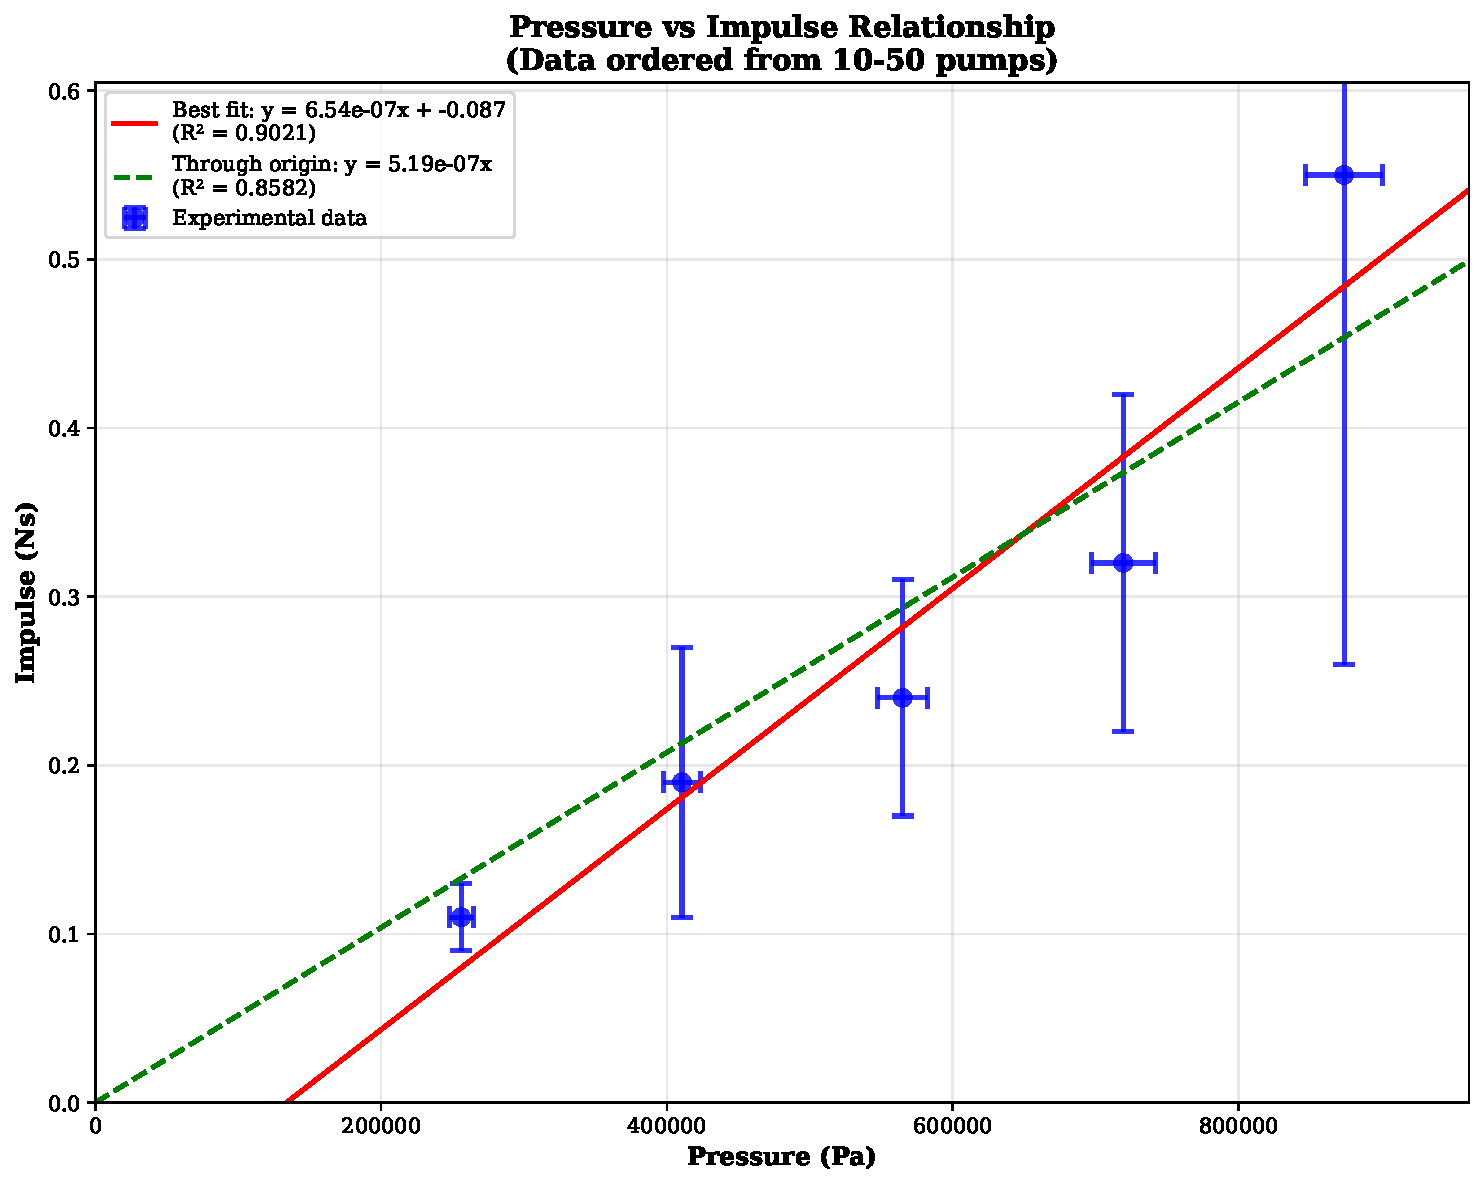
\includegraphics[width=0.95\textwidth]{pressure_vs_impulse_updated.pdf}
\caption{Pressure vs Impulse relationship with blue line of best fit and minimum/maximum bounds fixed at atmospheric pressure (1.016 × 10⁵ Pa)}
\label{fig:pressure_vs_impulse}
\end{figure}

\section{Key Findings}

\subsection{Line of Best Fit (Blue)}
The linear regression analysis shows a positive correlation between chamber pressure and impulse, indicating that higher chamber pressures result in greater impulse values.

\subsection{Error Bounds Analysis}
The minimum and maximum lines (green and orange dashed lines) represent the extreme possible relationships given the experimental uncertainties. These bounds:
\begin{itemize}
    \item Are anchored at atmospheric pressure (1.016 × 10⁵ Pa)
    \item Pass through the extreme points of the error bars
    \item Provide confidence intervals for the true relationship
    \item Show the range of possible slopes given measurement uncertainties
\end{itemize}

\subsection{Implications}
The consistent positive trend across all bounds confirms that chamber pressure has a significant positive impact on impulse generation, supporting the theoretical expectation that higher chamber pressures improve rocket engine performance.

\end{document}
